% Generated by Sphinx.
\def\sphinxdocclass{report}
\documentclass[a4paper,11pt,french]{rtdsphinxmanual}
\usepackage[utf8]{inputenc}
\DeclareUnicodeCharacter{00A0}{\nobreakspace}
\usepackage{cmap}
\usepackage[T1]{fontenc}
\usepackage[cyr]{aeguill}
\usepackage[francais]{babel}
\usepackage{times}
\usepackage[Bjornstrup]{fncychap}
\usepackage{longtable}
\usepackage{rtdsphinx}
\usepackage{multirow}

\addto\captionsfrench{\renewcommand{\figurename}{Fig. }}
\addto\captionsfrench{\renewcommand{\tablename}{Tableau }}
\floatname{literal-block}{Code source }



\title{Drupal 7}
\date{12 novembre 2015}
\release{1.0}
\author{Fabien Jarnet}
\newcommand{\sphinxlogo}{
\includegraphics[height=3cm]{logo.png}\par}
\renewcommand{\releasename}{Version}
\pagestyle{fancy}
\newcommand{\rtdbackgroundimage}{
\includegraphics[width=19cm]{latex_background_image.png}}
\newcommand{\rtdheaderbackgroundimage}{
\includegraphics[width=19cm]{latex_header_image.png}}
\newcommand{\rtdsubtitle}{DOCUMENTATION}
\newcommand{\rtdreference}{}
\newcommand{\rtdcopyright}{{Toute reproduction interdite sauf autorisation}}
\newcommand{\rtdfooterimage}{
\includegraphics[width=7cm]{latex_address.png}}
\makeindex[intoc]

\makeatletter
\def\PYG@reset{\let\PYG@it=\relax \let\PYG@bf=\relax%
    \let\PYG@ul=\relax \let\PYG@tc=\relax%
    \let\PYG@bc=\relax \let\PYG@ff=\relax}
\def\PYG@tok#1{\csname PYG@tok@#1\endcsname}
\def\PYG@toks#1+{\ifx\relax#1\empty\else%
    \PYG@tok{#1}\expandafter\PYG@toks\fi}
\def\PYG@do#1{\PYG@bc{\PYG@tc{\PYG@ul{%
    \PYG@it{\PYG@bf{\PYG@ff{#1}}}}}}}
\def\PYG#1#2{\PYG@reset\PYG@toks#1+\relax+\PYG@do{#2}}

\expandafter\def\csname PYG@tok@gd\endcsname{\def\PYG@tc##1{\textcolor[rgb]{0.63,0.00,0.00}{##1}}}
\expandafter\def\csname PYG@tok@gu\endcsname{\let\PYG@bf=\textbf\def\PYG@tc##1{\textcolor[rgb]{0.50,0.00,0.50}{##1}}}
\expandafter\def\csname PYG@tok@gt\endcsname{\def\PYG@tc##1{\textcolor[rgb]{0.00,0.27,0.87}{##1}}}
\expandafter\def\csname PYG@tok@gs\endcsname{\let\PYG@bf=\textbf}
\expandafter\def\csname PYG@tok@gr\endcsname{\def\PYG@tc##1{\textcolor[rgb]{1.00,0.00,0.00}{##1}}}
\expandafter\def\csname PYG@tok@cm\endcsname{\let\PYG@it=\textit\def\PYG@tc##1{\textcolor[rgb]{0.25,0.50,0.56}{##1}}}
\expandafter\def\csname PYG@tok@vg\endcsname{\def\PYG@tc##1{\textcolor[rgb]{0.73,0.38,0.84}{##1}}}
\expandafter\def\csname PYG@tok@m\endcsname{\def\PYG@tc##1{\textcolor[rgb]{0.13,0.50,0.31}{##1}}}
\expandafter\def\csname PYG@tok@mh\endcsname{\def\PYG@tc##1{\textcolor[rgb]{0.13,0.50,0.31}{##1}}}
\expandafter\def\csname PYG@tok@cs\endcsname{\def\PYG@tc##1{\textcolor[rgb]{0.25,0.50,0.56}{##1}}\def\PYG@bc##1{\setlength{\fboxsep}{0pt}\colorbox[rgb]{1.00,0.94,0.94}{\strut ##1}}}
\expandafter\def\csname PYG@tok@ge\endcsname{\let\PYG@it=\textit}
\expandafter\def\csname PYG@tok@vc\endcsname{\def\PYG@tc##1{\textcolor[rgb]{0.73,0.38,0.84}{##1}}}
\expandafter\def\csname PYG@tok@il\endcsname{\def\PYG@tc##1{\textcolor[rgb]{0.13,0.50,0.31}{##1}}}
\expandafter\def\csname PYG@tok@go\endcsname{\def\PYG@tc##1{\textcolor[rgb]{0.20,0.20,0.20}{##1}}}
\expandafter\def\csname PYG@tok@cp\endcsname{\def\PYG@tc##1{\textcolor[rgb]{0.00,0.44,0.13}{##1}}}
\expandafter\def\csname PYG@tok@gi\endcsname{\def\PYG@tc##1{\textcolor[rgb]{0.00,0.63,0.00}{##1}}}
\expandafter\def\csname PYG@tok@gh\endcsname{\let\PYG@bf=\textbf\def\PYG@tc##1{\textcolor[rgb]{0.00,0.00,0.50}{##1}}}
\expandafter\def\csname PYG@tok@ni\endcsname{\let\PYG@bf=\textbf\def\PYG@tc##1{\textcolor[rgb]{0.84,0.33,0.22}{##1}}}
\expandafter\def\csname PYG@tok@nl\endcsname{\let\PYG@bf=\textbf\def\PYG@tc##1{\textcolor[rgb]{0.00,0.13,0.44}{##1}}}
\expandafter\def\csname PYG@tok@nn\endcsname{\let\PYG@bf=\textbf\def\PYG@tc##1{\textcolor[rgb]{0.05,0.52,0.71}{##1}}}
\expandafter\def\csname PYG@tok@no\endcsname{\def\PYG@tc##1{\textcolor[rgb]{0.38,0.68,0.84}{##1}}}
\expandafter\def\csname PYG@tok@na\endcsname{\def\PYG@tc##1{\textcolor[rgb]{0.25,0.44,0.63}{##1}}}
\expandafter\def\csname PYG@tok@nb\endcsname{\def\PYG@tc##1{\textcolor[rgb]{0.00,0.44,0.13}{##1}}}
\expandafter\def\csname PYG@tok@nc\endcsname{\let\PYG@bf=\textbf\def\PYG@tc##1{\textcolor[rgb]{0.05,0.52,0.71}{##1}}}
\expandafter\def\csname PYG@tok@nd\endcsname{\let\PYG@bf=\textbf\def\PYG@tc##1{\textcolor[rgb]{0.33,0.33,0.33}{##1}}}
\expandafter\def\csname PYG@tok@ne\endcsname{\def\PYG@tc##1{\textcolor[rgb]{0.00,0.44,0.13}{##1}}}
\expandafter\def\csname PYG@tok@nf\endcsname{\def\PYG@tc##1{\textcolor[rgb]{0.02,0.16,0.49}{##1}}}
\expandafter\def\csname PYG@tok@si\endcsname{\let\PYG@it=\textit\def\PYG@tc##1{\textcolor[rgb]{0.44,0.63,0.82}{##1}}}
\expandafter\def\csname PYG@tok@s2\endcsname{\def\PYG@tc##1{\textcolor[rgb]{0.25,0.44,0.63}{##1}}}
\expandafter\def\csname PYG@tok@vi\endcsname{\def\PYG@tc##1{\textcolor[rgb]{0.73,0.38,0.84}{##1}}}
\expandafter\def\csname PYG@tok@nt\endcsname{\let\PYG@bf=\textbf\def\PYG@tc##1{\textcolor[rgb]{0.02,0.16,0.45}{##1}}}
\expandafter\def\csname PYG@tok@nv\endcsname{\def\PYG@tc##1{\textcolor[rgb]{0.73,0.38,0.84}{##1}}}
\expandafter\def\csname PYG@tok@s1\endcsname{\def\PYG@tc##1{\textcolor[rgb]{0.25,0.44,0.63}{##1}}}
\expandafter\def\csname PYG@tok@gp\endcsname{\let\PYG@bf=\textbf\def\PYG@tc##1{\textcolor[rgb]{0.78,0.36,0.04}{##1}}}
\expandafter\def\csname PYG@tok@sh\endcsname{\def\PYG@tc##1{\textcolor[rgb]{0.25,0.44,0.63}{##1}}}
\expandafter\def\csname PYG@tok@ow\endcsname{\let\PYG@bf=\textbf\def\PYG@tc##1{\textcolor[rgb]{0.00,0.44,0.13}{##1}}}
\expandafter\def\csname PYG@tok@sx\endcsname{\def\PYG@tc##1{\textcolor[rgb]{0.78,0.36,0.04}{##1}}}
\expandafter\def\csname PYG@tok@bp\endcsname{\def\PYG@tc##1{\textcolor[rgb]{0.00,0.44,0.13}{##1}}}
\expandafter\def\csname PYG@tok@c1\endcsname{\let\PYG@it=\textit\def\PYG@tc##1{\textcolor[rgb]{0.25,0.50,0.56}{##1}}}
\expandafter\def\csname PYG@tok@kc\endcsname{\let\PYG@bf=\textbf\def\PYG@tc##1{\textcolor[rgb]{0.00,0.44,0.13}{##1}}}
\expandafter\def\csname PYG@tok@c\endcsname{\let\PYG@it=\textit\def\PYG@tc##1{\textcolor[rgb]{0.25,0.50,0.56}{##1}}}
\expandafter\def\csname PYG@tok@mf\endcsname{\def\PYG@tc##1{\textcolor[rgb]{0.13,0.50,0.31}{##1}}}
\expandafter\def\csname PYG@tok@err\endcsname{\def\PYG@bc##1{\setlength{\fboxsep}{0pt}\fcolorbox[rgb]{1.00,0.00,0.00}{1,1,1}{\strut ##1}}}
\expandafter\def\csname PYG@tok@mb\endcsname{\def\PYG@tc##1{\textcolor[rgb]{0.13,0.50,0.31}{##1}}}
\expandafter\def\csname PYG@tok@ss\endcsname{\def\PYG@tc##1{\textcolor[rgb]{0.32,0.47,0.09}{##1}}}
\expandafter\def\csname PYG@tok@sr\endcsname{\def\PYG@tc##1{\textcolor[rgb]{0.14,0.33,0.53}{##1}}}
\expandafter\def\csname PYG@tok@mo\endcsname{\def\PYG@tc##1{\textcolor[rgb]{0.13,0.50,0.31}{##1}}}
\expandafter\def\csname PYG@tok@kd\endcsname{\let\PYG@bf=\textbf\def\PYG@tc##1{\textcolor[rgb]{0.00,0.44,0.13}{##1}}}
\expandafter\def\csname PYG@tok@mi\endcsname{\def\PYG@tc##1{\textcolor[rgb]{0.13,0.50,0.31}{##1}}}
\expandafter\def\csname PYG@tok@kn\endcsname{\let\PYG@bf=\textbf\def\PYG@tc##1{\textcolor[rgb]{0.00,0.44,0.13}{##1}}}
\expandafter\def\csname PYG@tok@o\endcsname{\def\PYG@tc##1{\textcolor[rgb]{0.40,0.40,0.40}{##1}}}
\expandafter\def\csname PYG@tok@kr\endcsname{\let\PYG@bf=\textbf\def\PYG@tc##1{\textcolor[rgb]{0.00,0.44,0.13}{##1}}}
\expandafter\def\csname PYG@tok@s\endcsname{\def\PYG@tc##1{\textcolor[rgb]{0.25,0.44,0.63}{##1}}}
\expandafter\def\csname PYG@tok@kp\endcsname{\def\PYG@tc##1{\textcolor[rgb]{0.00,0.44,0.13}{##1}}}
\expandafter\def\csname PYG@tok@w\endcsname{\def\PYG@tc##1{\textcolor[rgb]{0.73,0.73,0.73}{##1}}}
\expandafter\def\csname PYG@tok@kt\endcsname{\def\PYG@tc##1{\textcolor[rgb]{0.56,0.13,0.00}{##1}}}
\expandafter\def\csname PYG@tok@sc\endcsname{\def\PYG@tc##1{\textcolor[rgb]{0.25,0.44,0.63}{##1}}}
\expandafter\def\csname PYG@tok@sb\endcsname{\def\PYG@tc##1{\textcolor[rgb]{0.25,0.44,0.63}{##1}}}
\expandafter\def\csname PYG@tok@k\endcsname{\let\PYG@bf=\textbf\def\PYG@tc##1{\textcolor[rgb]{0.00,0.44,0.13}{##1}}}
\expandafter\def\csname PYG@tok@se\endcsname{\let\PYG@bf=\textbf\def\PYG@tc##1{\textcolor[rgb]{0.25,0.44,0.63}{##1}}}
\expandafter\def\csname PYG@tok@sd\endcsname{\let\PYG@it=\textit\def\PYG@tc##1{\textcolor[rgb]{0.25,0.44,0.63}{##1}}}

\def\PYGZbs{\char`\\}
\def\PYGZus{\char`\_}
\def\PYGZob{\char`\{}
\def\PYGZcb{\char`\}}
\def\PYGZca{\char`\^}
\def\PYGZam{\char`\&}
\def\PYGZlt{\char`\<}
\def\PYGZgt{\char`\>}
\def\PYGZsh{\char`\#}
\def\PYGZpc{\char`\%}
\def\PYGZdl{\char`\$}
\def\PYGZhy{\char`\-}
\def\PYGZsq{\char`\'}
\def\PYGZdq{\char`\"}
\def\PYGZti{\char`\~}
% for compatibility with earlier versions
\def\PYGZat{@}
\def\PYGZlb{[}
\def\PYGZrb{]}
\makeatother

\renewcommand\PYGZsq{\textquotesingle}

\begin{document}

\maketitle
\tableofcontents
\phantomsection\label{index::doc}



\chapter{Poste de travail}
\label{poste_travail:drupal-7}\label{poste_travail::doc}\label{poste_travail:poste-de-travail}

\section{Emplacement des sources}
\label{poste_travail:emplacement-des-sources}
Comme pour eZPublish, les sources sont séparées en 2 :
\begin{itemize}
\item {} 
\code{/data/sources/site} : code source versionné du projet

\item {} 
\code{/data/services/web/site} : instance Drupal du projet

\end{itemize}

Des liens symboliques s'effectuent entre les 2 pour faciliter le développement et le déploiement.

{\hfill\scalebox{0.900000}{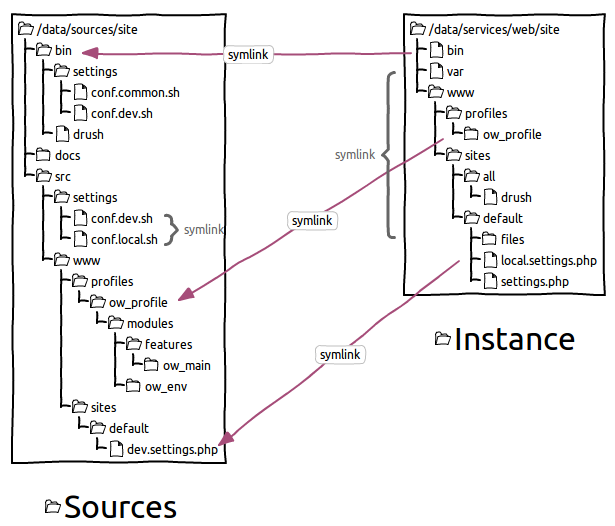
\includegraphics{arbo.png}}\hfill}


\section{Description de l'arborescence}
\label{poste_travail:description-de-l-arborescence}\begin{itemize}
\item {} \begin{description}
\item[{\code{bin/}}] \leavevmode{[}submodule Open Wide permettant de déployer un environnement.{]}\begin{itemize}
\item {} 
\code{bin/settings/} : configuration globale + fichiers init de copie d'environnement nécessaire lors de l'install

\item {} 
\code{bin/vendor/} : drush (+ autres outils uniquement en local comme le code sniffer, phpmd)

\end{itemize}

\end{description}

\item {} \begin{description}
\item[{\code{src/}}] \leavevmode{[}code source spécifique{]}\begin{itemize}
\item {} 
\code{src/settings/drush/} : versions de modules/thèmes activés/désactivés selon un environnement

\item {} 
\code{src/www/profiles/ow\_profile/} : profil d'installation contenant les modules et thèmes spécifiques utilisés sur le site

\item {} 
\code{src/www/sites/default/} : configuration spécifique à un environnement (inclus à la fin de \code{settings.php})

\end{itemize}

\end{description}

\item {} 
\code{www/} : lien symbolique de l'instance du site Drupal (permet de lancer des commandes drush depuis les sources)

\end{itemize}


\section{PHP Storm}
\label{poste_travail:php-storm}

\subsection{Code Sniffer}
\label{poste_travail:code-sniffer}
Pour coder sur Drupal, il faut développer selon certaines conventions de codage.

Dans le module \textbf{coder} se trouve le \textbf{PHP Code Sniffer} qui propose toutes les règles d'écriture spécifiques à Drupal.

Restera à la référencer dans votre IDE préféré.
\begin{itemize}
\item {} 
Aller dans le menu \code{Settings \textgreater{} Editor \textgreater{} Inspections}

\item {} 
Cocher \code{PHP \textgreater{} PHP Code Sniffer validation} puis sélectionner dans les options le \emph{Coding standard} \textbf{Custom}

\item {} 
Parcourir l'arborescence pour aller jusqu'au module Drupal \code{coder} de votre projet (\emph{{[}PROJECT\_DIRECTORY{]}/www/sites/all/modules/contrib/coder/coder\_sniffer/Drupal/})

\item {} 
Aller dans le menu \code{Settings \textgreater{} Languages \& Frameworks \textgreater{} PHP \textgreater{} Code Sniffer}

\item {} 
Dans le chemin du phpcs, parcourir l'arborescence d'un de vos projets, puis sélectionnez l'exécutable dans le submodule : \emph{{[}PROJECT\_DIRECTORY{]}/bin/vendor/bin/phpcs}

\end{itemize}


\strong{Voir aussi:}

\begin{itemize}
\item {} 
Paramétrage PHPStorm Drupal : \href{https://www.drupal.org/node/1962108}{https://www.drupal.org/node/1962108}

\item {} 
Utilisation de PHPStorm pour Drupal : \href{https://confluence.jetbrains.com/display/PhpStorm/Drupal+Development+using+PhpStorm}{https://confluence.jetbrains.com/display/PhpStorm/Drupal+Development+using+PhpStorm}

\item {} 
Installation Code Sniffer : \href{https://confluence.jetbrains.com/display/PhpStorm/PHP+Code+Sniffer+in+PhpStorm}{https://confluence.jetbrains.com/display/PhpStorm/PHP+Code+Sniffer+in+PhpStorm}

\end{itemize}




\subsection{Behat}
\label{poste_travail:behat}
Installez le plugin \textbf{Behat} pour activer la coloration syntaxique des fichiers \emph{.feature}.


\chapter{Installation}
\label{installation:installation}\label{installation::doc}

\section{Pré-requis}
\label{installation:pre-requis}
\begin{Verbatim}[commandchars=\\\{\}]
\PYG{c}{\PYGZsh{} Pour dézipper les libraires JS téléchargées}
\PYG{n+nv}{\PYGZdl{} }sudo apt\PYGZhy{}get install unzip

\PYG{c}{\PYGZsh{} Génération de la documentation Sphinx en PDF}
\PYG{n+nv}{\PYGZdl{} }sudo apt\PYGZhy{}get install texlive
\end{Verbatim}


\section{Création initiale du projet}
\label{installation:creation-initiale-du-projet}
\begin{notice}{attention}{Attention:}
Cette phase n'est nécessaire que lors du démarrage d'un projet. Si le projet a déjà un repository, alors passez directement à l'étape suivante {\hyperref[installation:installation-projet]{\emph{installation-projet}}}.
\end{notice}


\subsection{Installation du repository OWSI-Drupal 7}
\label{installation:installation-du-repository-owsi-drupal-7}
\begin{Verbatim}[commandchars=\\\{\}]
\PYG{n+nv}{\PYGZdl{} }\PYG{n+nb}{cd} /data/sources
\PYG{n+nv}{\PYGZdl{} }git clone ssh://git.projects.openwide.fr/gitroot/owsi\PYGZhy{}drupal7
\PYG{n+nv}{\PYGZdl{} }\PYG{n+nb}{cd} /data/sources/owsi\PYGZhy{}drupal7
\PYG{n+nv}{\PYGZdl{} }git submodule update \PYGZhy{}\PYGZhy{}init
\end{Verbatim}


\subsection{Initialisation du projet}
\label{installation:initialisation-du-projet}
Clônez le repository du projet dans \emph{{[}PROJECT\_DIRECTORY{]}}, puis lancez le script d'initialisation \textbf{à partir du dossier owsi-drupal7} :

\begin{Verbatim}[commandchars=\\\{\}]
\PYG{n+nv}{\PYGZdl{} }\PYG{n+nb}{cd} /data/sources/owsi\PYGZhy{}drupal7/bin
\PYG{n+nv}{\PYGZdl{} }chmod u+x create\PYGZhy{}project.sh
\PYG{n+nv}{\PYGZdl{} }./create\PYGZhy{}project.sh \PYG{o}{[}PROJECT\PYGZus{}DIRECTORY\PYG{o}{]}
\end{Verbatim}


\section{Installation du projet}
\label{installation:installation-projet}\label{installation:installation-du-projet}

\subsection{Création du VHost}
\label{installation:creation-du-vhost}
Configurez votre VHost comme ceci :

\begin{Verbatim}[commandchars=\\\{\}]
\PYG{n+nt}{\PYGZlt{}VirtualHost} \PYG{l+s}{*:80}\PYG{n+nt}{\PYGZgt{}}

    \PYG{n+nt}{\PYGZlt{}Directory} \PYG{l+s}{/data/services/web/MY\PYGZus{}PROJECT/www}\PYG{n+nt}{\PYGZgt{}}
        \PYG{n+nb}{Require} \PYG{k}{all} granted
        \PYG{n+nb}{Options} FollowSymLinks
        \PYG{n+nb}{AllowOverride} \PYG{k}{All}
    \PYG{n+nt}{\PYGZlt{}/Directory}\PYG{n+nt}{\PYGZgt{}}

    \PYG{n+nb}{ServerAdmin} webmaster@example.fr
    \PYG{n+nb}{DocumentRoot} \PYG{l+s+sx}{/data/services/web/MY\PYGZus{}PROJECT/www}
    \PYG{n+nb}{ServerName} www.MY\PYGZus{}PROJECT.loc
    \PYG{n+nb}{ServerAlias} MY\PYGZus{}PROJECT.loc
    \PYG{n+nb}{RewriteEngine} \PYG{k}{On}
    \PYG{n+nb}{RewriteOptions} inherit
    \PYG{n+nb}{CustomLog} \PYG{l+s+sx}{/var/log/apache2/MY\PYGZus{}PROJECT.log} combined

\PYG{n+nt}{\PYGZlt{}/VirtualHost}\PYG{n+nt}{\PYGZgt{}}
\end{Verbatim}


\subsection{Création de la BDD}
\label{installation:creation-de-la-bdd}
Créez la BDD via phpMyAdmin ou en ligne de commandes :

\begin{Verbatim}[commandchars=\\\{\}]
\PYG{n+nv}{\PYGZdl{} }mysql \PYGZhy{}u \PYG{o}{[}username\PYG{o}{]} \PYGZhy{}e \PYG{l+s+s2}{\PYGZdq{}CREATE DATABASE \PYGZus{}\PYGZus{}db\PYGZus{}\PYGZus{} CHARACTER SET utf8 COLLATE utf8\PYGZus{}general\PYGZus{}ci;\PYGZdq{}}
\PYG{n+nv}{\PYGZdl{} }mysql \PYGZhy{}u \PYG{o}{[}username\PYG{o}{]}\PYG{p}{;}
\end{Verbatim}

Puis affectez les droits à un user MySQL que vousdoc créerez :

\begin{Verbatim}[commandchars=\\\{\}]
\PYG{k}{GRANT} \PYG{k}{SELECT}\PYG{p}{,} \PYG{k}{INSERT}\PYG{p}{,} \PYG{k}{UPDATE}\PYG{p}{,} \PYG{k}{DELETE}\PYG{p}{,} \PYG{k}{CREATE}\PYG{p}{,} \PYG{k}{DROP}\PYG{p}{,} \PYG{k}{INDEX}\PYG{p}{,} \PYG{k}{ALTER}\PYG{p}{,} \PYG{k}{CREATE} \PYG{n}{TEMPORARY} \PYG{k+kp}{TABLES} \PYG{k}{ON} \PYG{n}{\PYGZus{}\PYGZus{}db\PYGZus{}\PYGZus{}}\PYG{p}{.}\PYG{o}{*} \PYG{k}{TO} \PYG{l+s+s1}{\PYGZsq{}admin\PYGZsq{}}\PYG{o}{@}\PYG{l+s+s1}{\PYGZsq{}localhost\PYGZsq{}} \PYG{n}{IDENTIFIED} \PYG{k}{BY} \PYG{l+s+s1}{\PYGZsq{}admin\PYGZsq{}}\PYG{p}{;}
\end{Verbatim}


\strong{Voir aussi:}


Création de la BDD : \href{https://www.drupal.org/documentation/install/create-database}{https://www.drupal.org/documentation/install/create-database}




\subsection{Installation du site}
\label{installation:installation-du-site}

\subsubsection{Introduction}
\label{installation:introduction}
\textbf{Que fait l'installeur ?}
\begin{itemize}
\item {} 
Récupération de Drush via composer

\item {} 
Génération des fichiers de settings nécessaires :
\begin{itemize}
\item {} 
\emph{drush.env.php/drush.common.php} : Activation/désactivation des modules/thèmes/settings de façon générale ou par environnement (dev, recette, prod ...)

\item {} 
\emph{conf.{[}env{]}.sh} : Paramétrage de l'environnement courant avec les accès SSH / répertoires d'installation

\item {} 
\emph{sites/{[}site{]}/common.settings.php} / \emph{sites/{[}site{]}/{[}env{]}.settings.php} : Configuration de la BDD de chaque site (cas du multisite)

\end{itemize}

\item {} 
Création des répertoires / liens symboliques nécéssaires dans le répertoire de travail / instance Drupal

\item {} 
Utilisation du profil \emph{Ow Profile} comme base pour les modules/thèmes spécifiques sur le site

\item {} 
Récupération du core Drupal + création de la BDD

\item {} 
Récupération et copie des librairies JS distantes indiquées dans le fichier \code{ow\_profile.make} du profil

\item {} 
Application des droits de lecture/écriture selon les préconisations Drupal.org

\item {} 
Insertion de variables custom dans la console d'administration générale Drupal

\end{itemize}


\subsubsection{Lancement}
\label{installation:lancement}
Clônez le repository du projet dans votre workspace :

\begin{Verbatim}[commandchars=\\\{\}]
\PYG{n+nv}{\PYGZdl{} }\PYG{n+nb}{cd} /data/sources/
\PYG{n+nv}{\PYGZdl{} }git clone ssh://git.projects.openwide.fr/gitroot/MY\PYGZus{}PROJECT
\PYG{n+nv}{\PYGZdl{} }\PYG{n+nb}{cd} /data/sources/MY\PYGZus{}PROJECT
\PYG{n+nv}{\PYGZdl{} }git submodule update \PYGZhy{}\PYGZhy{}init
\PYG{n+nv}{\PYGZdl{} }./bin/install.sh \PYGZhy{}e dev
\end{Verbatim}

\begin{notice}{note}{Note:}
Lors de la saisie des paramètres de BDD \& co sur les environnements distants, copiez-les également dans le wiki OW ou dans un doc sphinx interne pour historique.
\end{notice}


\subsection{Traductions}
\label{installation:traductions}
Allez dans l'interface d'administration, et appliquez la langue par défaut pour le BO : \href{http://myvhost.loc/admin/config/regional/language}{http://myvhost.loc/admin/config/regional/language}, puis lancez la commande de mise à jour des traductions du core et des modules :

\begin{Verbatim}[commandchars=\\\{\}]
\PYG{n+nv}{\PYGZdl{} }./bin/drush l10n\PYGZhy{}update\PYGZhy{}refresh
\PYG{n+nv}{\PYGZdl{} }./bin/drush l10n\PYGZhy{}update
\end{Verbatim}

\begin{notice}{note}{Note:}
Le temps de chargement peut être relativement long alors ... allez chercher un café ;-)
\end{notice}


\chapter{Environnements}
\label{environnement:environnements}\label{environnement::doc}

\section{Modules}
\label{environnement:modules}
Installer les modules pour l'environnement courant :

\begin{Verbatim}[commandchars=\\\{\}]
\PYG{n+nv}{\PYGZdl{} }\PYG{n+nb}{cd} /data/sources/owsi\PYGZhy{}drupal7/bin
\PYG{n+nv}{\PYGZdl{} }./bin/drush environment \PYGZhy{}y
\end{Verbatim}

Ce script va mettre à jour la BDD locale selon les informations saisies dans les fichiers \code{src/www/sites/all/drush/drush\_settings/drush.common.php} et \code{src/www/sites/all/drush/drush\_settings/drush.{[}CURRENT\_ENV{]}.php}


\section{Nouvel environnement}
\label{environnement:nouvel-environnement}
Cas : Je souhaite créer les settings pour l'environnement de \textbf{prod}.

\begin{Verbatim}[commandchars=\\\{\}]
\PYG{n+nv}{\PYGZdl{} }\PYG{n+nb}{cd} /data/sources/owsi\PYGZhy{}drupal7/bin
\PYG{n+nv}{\PYGZdl{} }./create\PYGZhy{}env.sh prod
\end{Verbatim}

Des fichiers seront initialisés à partir des fichiers exemples, la liste apparaîtra à l'écran au lancement de la commande.


\chapter{Commandes Drush}
\label{drush::doc}\label{drush:commandes-drush}

\section{Autocomplétion}
\label{drush:autocompletion}
Pour faciliter l'écriture de commandes Drush, il existe un outil d'autocomplétion.


\strong{Voir aussi:}


\href{http://developpeur-drupal.com/article/drush-avance-installation-composer-alias-autocompletions}{http://developpeur-drupal.com/article/drush-avance-installation-composer-alias-autocompletions}




\section{Activer un module}
\label{drush:activer-un-module}
Si le module n'est pas dans les sources, alors il est téléchargé dans sa dernière version compatible avec le core choisi par le profil (ex : 7.x).

Cependant, avant de télécharger la dernière version d'un module, il est conseillé de le tester en local pour vérifier qu'il n'y a pas de régression.

On utilisera le module \textbf{update\_manager} pour être averti en BO des nouvelles versions des modules installés.

\begin{Verbatim}[commandchars=\\\{\}]
\PYG{n+nv}{\PYGZdl{} }./bin/drush en mymodule
\end{Verbatim}


\section{Désactiver un module}
\label{drush:desactiver-un-module}
\begin{Verbatim}[commandchars=\\\{\}]
\PYG{n+nv}{\PYGZdl{} }./bin/drush dis mymodule
\end{Verbatim}


\section{Lister les modules du site}
\label{drush:lister-les-modules-du-site}
\begin{Verbatim}[commandchars=\\\{\}]
\PYG{n+nv}{\PYGZdl{} }./bin/drush pml
\end{Verbatim}


\section{Dumper une BDD}
\label{drush:dumper-une-bdd}
\begin{Verbatim}[commandchars=\\\{\}]
\PYG{n+nv}{\PYGZdl{} }./bin/drush sql\PYGZhy{}dump \PYGZgt{} dump.sql
\end{Verbatim}


\section{Vider le cache}
\label{drush:vider-le-cache}
\begin{Verbatim}[commandchars=\\\{\}]
\PYG{n+nv}{\PYGZdl{} }./bin/drush cc all
\PYG{n+nv}{\PYGZdl{} }./bin/drush cc css\PYGZhy{}js
\end{Verbatim}


\section{Mettre à jour une BDD}
\label{drush:mettre-a-jour-une-bdd}
Met à jour la BDD selon les hooks créés

\begin{Verbatim}[commandchars=\\\{\}]
\PYG{n+nv}{\PYGZdl{} }./bin/drush updb
\end{Verbatim}


\section{Mode maintenance}
\label{drush:mode-maintenance}
\begin{Verbatim}[commandchars=\\\{\}]
\PYG{n+nv}{\PYGZdl{} }./bin/drush vset maintenance\PYGZus{}mode 1
\PYG{n+nv}{\PYGZdl{} }./bin/drush vset maintenance\PYGZus{}mode 0
\end{Verbatim}


\section{Gestion du cache des alias d'image}
\label{drush:gestion-du-cache-des-alias-d-image}
Regénère le itok des images

\begin{Verbatim}[commandchars=\\\{\}]
\PYG{n+nv}{\PYGZdl{} }./bin/drush vset drupal\PYGZus{}private\PYGZus{}key 0
\PYG{n+nv}{\PYGZdl{} }rm \PYGZhy{}rf sites/default/files/styles/\PYG{o}{[}STYLE\PYGZus{}NAME\PYG{o}{]}/*
\end{Verbatim}


\section{Debug}
\label{drush:debug}
\begin{Verbatim}[commandchars=\\\{\}]
\PYG{n+nv}{\PYGZdl{} }./bin/drush ws \PYGZhy{}\PYGZhy{}tail
\end{Verbatim}


\section{Features}
\label{drush:features}

\strong{Voir aussi:}


\href{http://drupalfr.org/documentation/prise-main-detaillee-modules-context-features}{http://drupalfr.org/documentation/prise-main-detaillee-modules-context-features}




\subsection{features-update}
\label{drush:features-update}
Appliquer les modifications de la BDD dans le fichier.

Cas : On a mis à jour les droits utilisateurs ou un type de contenu en local, on lance cette commande pour injecter les modifications dans la feature pour déploiement sur les environnements

\begin{Verbatim}[commandchars=\\\{\}]
\PYG{n+nv}{\PYGZdl{} }./bin/drush fu \PYGZhy{}y ow\PYGZus{}main
\end{Verbatim}


\subsection{features-revert}
\label{drush:features-revert}
Appliquer les modifications fichiers dans la BDD.

Cas : On déploie des modifications sur les environnements (Attention : écrase les valeurs précédemments affectées)

\begin{Verbatim}[commandchars=\\\{\}]
\PYG{n+nv}{\PYGZdl{} }./bin/drush fr \PYGZhy{}y ow\PYGZus{}main
\PYG{n+nv}{\PYGZdl{} }./bin/drush fra \PYG{o}{(}features\PYGZhy{}revert\PYGZhy{}all\PYG{o}{)}
\end{Verbatim}


\subsection{features-export}
\label{drush:features-export}
Pour exporter une variable dans le fichier \code{module.info} du module

\begin{Verbatim}[commandchars=\\\{\}]
\PYG{c}{\PYGZsh{} ./bin/drush fe mymodule var:googleanalytics\PYGZus{}account}
\PYG{n+nv}{\PYGZdl{} }./bin/drush fe mymodule my\PYGZus{}variable
\end{Verbatim}


\strong{Voir aussi:}


\href{https://www.drupal.org/node/960926}{https://www.drupal.org/node/960926}

\href{http://docs.drush.org/en/master/examples/}{http://docs.drush.org/en/master/examples/}

\href{http://drewpull.drupalgardens.com/blog/drush-make-site-deployment}{http://drewpull.drupalgardens.com/blog/drush-make-site-deployment}




\chapter{Les modules}
\label{modules:les-modules}\label{modules::doc}

\section{Modules du core}
\label{modules:modules-du-core}
Voici un descriptif de quelques modules du core :
\begin{itemize}
\item {} 
\code{aggregator} : Gestion de flux RSS

\item {} 
\code{block} : Fournit les outils pour créer des blocks dans des régions d'un thème

\item {} 
\code{color} : Permet de customiser les couleurs des thèmes compatibles

\item {} 
\code{comment} : Autorise les utilisateurs à commenter des contenus

\item {} 
\code{contact} : Module de contact standard

\item {} 
\code{field} / \code{field\_ui} : API de manipulations de champs

\item {} 
\code{file} : Field type Fichier

\item {} 
\code{image} : Field type image + gestion des alias

\item {} 
\code{locale} : Permet de traduire l'interface dans plusieurs langues

\item {} 
\code{list} : Field type Liste

\item {} 
\code{number} : Field type Nombre

\item {} 
\code{options} : Field type Options (selection/checkbox/radio)

\item {} 
\code{poll} : Gestion d'un sondage simple

\item {} 
\code{statistics} : Enregistrement des statistiques de consultation dans Drupal

\item {} 
\code{taxonomy} : Permet d'utiliser la taxonomie

\end{itemize}


\section{Modules additionnels}
\label{modules:modules-additionnels}
Voici une liste non exhaustive des modules additionnels utiles :
\begin{itemize}
\item {} 
\code{admin\_menu} : Menu d'administration multi-niveaux plus pratique que le menu de base - \href{https://www.drupal.org/project/admin\_menu}{https://www.drupal.org/project/admin\_menu}

\item {} 
\code{boost} : Génère du page statique pour le trafic anonyme - \href{https://www.drupal.org/project/boost}{https://www.drupal.org/project/boost}

\item {} 
\code{captcha} : Image captcha avec caractères à saisir - \href{https://www.drupal.org/project/captcha}{https://www.drupal.org/project/captcha}

\item {} 
\code{ckeditor} : Fournit un RTE paramétrable pour le contributeur - \href{https://www.drupal.org/project/ckeditor}{https://www.drupal.org/project/ckeditor}

\item {} 
\code{coder} : Fournit PHP\_CodeSniffer - \href{https://www.drupal.org/project/coder}{https://www.drupal.org/project/coder}

\item {} 
\code{ctools} : Fournit des outils utilisés par plusieurs modules facilitant le développement - \href{https://www.drupal.org/project/ctools}{https://www.drupal.org/project/ctools}

\item {} 
\code{date} : Field type Date - \href{https://www.drupal.org/project/date}{https://www.drupal.org/project/date}

\item {} 
\code{devel} : Fonctions/helpers de développement pour le debug - \href{https://www.drupal.org/project/devel}{https://www.drupal.org/project/devel}

\item {} 
\code{email} : Field type Email - \href{https://www.drupal.org/project/email}{https://www.drupal.org/project/email}

\item {} 
\code{entity} : Fournit des fonctions pour manipuler les entités via le code (create / save / delete / view / access) - \href{https://www.drupal.org/project/entity}{https://www.drupal.org/project/entity}

\item {} 
\code{entitycache} : Place les requêtes BDD des entités du core en cache

\item {} 
\code{features} : Permet d'importer/exporter des entités, settings, et autres paramétrages entre plusieurs environnements - \href{https://www.drupal.org/project/features}{https://www.drupal.org/project/features}

\item {} 
\code{field\_permissions} : Permissions sur des champs - \href{https://www.drupal.org/project/field\_permissions}{https://www.drupal.org/project/field\_permissions}

\item {} 
\code{globalredirect} : Fournit une liste de règles de redirection de base - \href{https://www.drupal.org/project/globalredirect}{https://www.drupal.org/project/globalredirect}

\item {} 
\code{honeypot} : Honeypot pour formulaires - \href{https://www.drupal.org/project/honeypot}{https://www.drupal.org/project/honeypot}

\item {} 
\code{imagecache\_actions} : Mise à disposition de filtres d'images supplémentaires - \href{https://www.drupal.org/project/imagecache\_actions}{https://www.drupal.org/project/imagecache\_actions}

\item {} 
\code{imce} : Téléchargement de medias dans un browser - \href{https://www.drupal.org/project/imce}{https://www.drupal.org/project/imce}

\item {} 
\code{l10n\_client} : Fournit un bouton en bas à droite qui permet de détecter les traductions sur la page courante - \href{https://www.drupal.org/project/l10n\_client}{https://www.drupal.org/project/l10n\_client}. /!Version jQuery \textless{} 1.9 (support de \$.browser)

\item {} 
\code{l10n\_update} : Permet de mettre à jour les traductions de tous les modules - \href{https://www.drupal.org/project/l10n\_update}{https://www.drupal.org/project/l10n\_update}

\item {} 
\code{jquery\_update} : \href{https://www.drupal.org/project/jquery\_update}{https://www.drupal.org/project/jquery\_update}

\item {} 
\code{link} : Field type Lien - \href{https://www.drupal.org/project/link}{https://www.drupal.org/project/link}

\item {} 
\code{linkit} : Fournit un menu ajax lors de la saisie d'un node en relation - \href{https://www.drupal.org/project/linkit}{https://www.drupal.org/project/linkit}

\item {} 
\code{maillog} : Simule l'envoi d'un mail pour affichage dans le flux/BDD uniquement (mode dev sur données de prod) - \href{https://www.drupal.org/project/maillog}{https://www.drupal.org/project/maillog}

\item {} 
\code{media} : Management des media - \href{https://www.drupal.org/project/media}{https://www.drupal.org/project/media}

\item {} 
\code{menu\_block} : Fournit des blocks menu de niveaux inférieurs - \href{https://www.drupal.org/project/menu\_block}{https://www.drupal.org/project/menu\_block}

\item {} 
\code{metatag} : - \href{https://www.drupal.org/project/metatag}{https://www.drupal.org/project/metatag}

\item {} 
\code{migrate} : Import de données depuis Drupal 5/6/7, Wordpress ou autres - \href{https://www.drupal.org/project/migrate}{https://www.drupal.org/project/migrate}

\item {} 
\code{module\_filter} : Améliore l'interface d'administration des modules - \href{https://www.drupal.org/project/module\_filter}{https://www.drupal.org/project/module\_filter}

\item {} 
\code{pathauto} : Génère automatiquement des alias d'URL selon l'entité (+ règles paramétrables par type de contenu) - \href{https://www.drupal.org/project/pathauto}{https://www.drupal.org/project/pathauto}

\item {} 
\code{print} : Génération d'une version imprimable web/pdf/epub/email - \href{https://www.drupal.org/project/print}{https://www.drupal.org/project/print}

\item {} 
\code{redirect} : Améliore la gestion des redirections - \href{https://www.drupal.org/project/redirect}{https://www.drupal.org/project/redirect}

\item {} 
\code{rules} : \href{https://www.drupal.org/project/rules}{https://www.drupal.org/project/rules}

\item {} 
\code{search\_api} : \href{https://www.drupal.org/project/search\_api}{https://www.drupal.org/project/search\_api}

\item {} 
\code{security\_review} : Fournit une batterie de tests basiques de sécurité - \href{https://www.drupal.org/project/security\_review}{https://www.drupal.org/project/security\_review}

\item {} 
\code{special\_menu\_items} : Permet d'ajouter des entrées de menu sans lien ou séparateurs - \href{https://www.drupal.org/project/special\_menu\_items}{https://www.drupal.org/project/special\_menu\_items}

\item {} 
\code{strongarm} : Permet d'importer/exporter des variables depuis des fichiers ou BDD (fonctionne avec features) - \href{https://www.drupal.org/project/strongarm}{https://www.drupal.org/project/strongarm}

\item {} 
\code{taxonomy\_menu} : Transforme l'arbo des termes en menu  - \href{https://www.drupal.org/project/taxonomy\_menu}{https://www.drupal.org/project/taxonomy\_menu}

\item {} 
\code{token} : \href{https://www.drupal.org/project/token}{https://www.drupal.org/project/token}

\item {} 
\code{transliteration} : Transformation de chaines pour génération d'URL propres si caractères spéciaux (ou dans une langue spécifique) - \href{https://www.drupal.org/project/transliteration}{https://www.drupal.org/project/transliteration}

\item {} 
\code{xmlsitemap} : \href{https://www.drupal.org/project/xmlsitemap}{https://www.drupal.org/project/xmlsitemap}

\end{itemize}


\section{Autres modules}
\label{modules:autres-modules}\begin{itemize}
\item {} 
\code{webform} : Création de formulaire au clic interface

\item {} 
\code{poll} ou \code{advanced\_poll}

\item {} 
\code{migrate} : API riche en objet avec la prise en compte de migration depuis Joomla / Wordpress ... - \href{https://www.drupal.org/project/migrate}{https://www.drupal.org/project/migrate}

\item {} 
\code{feeds} : \href{https://www.drupal.org/project/feeds}{https://www.drupal.org/project/feeds}

\end{itemize}


\section{Arbo d'un module}
\label{modules:arbo-d-un-module}\begin{itemize}
\item {} 
\code{mymodule.info} : Metadonnées du module : lister des fichiers PHP objet/interface dans files{[}{]}, stylesheets{[}all{]} ou scripts{[}{]} chargé partout / Vider le cache de Drupal si on le modifie

\item {} 
\code{mymodule.module} : Liste des hooks

\item {} 
\code{mymodule.install} : Code d'install / désinstall / mise à jour nécessaire

\item {} 
\code{*.js} : à référencer avec drupal\_add\_js()

\item {} 
\code{*.css} : à référencer avec drupal\_add\_css()

\item {} 
\code{*.inc} : Code PHP supplémentaires si besoin : à inclure avec require / module\_load\_include() ...

\end{itemize}


\chapter{Les thèmes}
\label{themes:les-themes}\label{themes::doc}

\section{Thèmes d'administration}
\label{themes:themes-d-administration}\begin{itemize}
\item {} 
\code{adminimal\_theme} : Thème d'administration alternatif - \href{https://www.drupal.org/project/adminimal\_theme}{https://www.drupal.org/project/adminimal\_theme}

\end{itemize}


\section{Thèmes front}
\label{themes:themes-front}\begin{itemize}
\item {} 
\code{bootstrap} : Thème sur Bootstrap 3 - \href{https://www.drupal.org/project/bootstrap}{https://www.drupal.org/project/bootstrap}

\end{itemize}


\chapter{Theming}
\label{theming::doc}\label{theming:theming}

\section{Fonctions de base}
\label{theming:fonctions-de-base}\begin{itemize}
\item {} 
\code{drupal\_get\_path()} : pour récupérer chaque chemin de fichier css/js

\item {} 
\code{drupal\_add\_css()} : groupe CSS\_DEFAULT / CSS\_THEME

\end{itemize}


\section{Hooks}
\label{theming:hooks}\begin{itemize}
\item {} 
\code{hook\_block\_view()} : Drupal sapprête à afficherun bloc - \href{https://api.drupal.org/hook\_block\_view}{https://api.drupal.org/hook\_block\_view}

\item {} 
\code{hook\_user\_login()} : Quand l'utilisateur s'authentifie - \href{https://api.drupal.org/hook\_user\_login}{https://api.drupal.org/hook\_user\_login}

\item {} 
\code{hook\_form\_alter()} : Avant qu'un formulaire soit affiché - \href{https://api.drupal.org/hook\_form\_alter}{https://api.drupal.org/hook\_form\_alter}

\item {} 
\code{hook\_block\_info()} : Déclaration de nouveaux blocks - \href{https://api.drupal.org/hook\_block\_info}{https://api.drupal.org/hook\_block\_info}

\item {} 
\code{hook\_node\_validate()} : \href{https://api.drupal.org/hook\_node\_validate}{https://api.drupal.org/hook\_node\_validate}

\item {} 
\code{hook\_node\_insert()} : \href{https://api.drupal.org/hook\_node\_insert}{https://api.drupal.org/hook\_node\_insert}

\item {} 
\code{hook\_node\_update()} : \href{https://api.drupal.org/hook\_node\_update}{https://api.drupal.org/hook\_node\_update}

\item {} 
\code{hook\_node\_detete()} : \href{https://api.drupal.org/hook\_node\_detete}{https://api.drupal.org/hook\_node\_detete}

\item {} 
\code{hook\_menu()} : \href{https://api.drupal.org/hook\_menu}{https://api.drupal.org/hook\_menu}

\end{itemize}


\section{Infos}
\label{theming:infos}\begin{itemize}
\item {} 
Si plusieurs hook \emph{titi\_block\_view}/\emph{toto\_block\_view} sont appelés, l'ordre d'appel est par ordre alphabétique. Si on veut contourner, on change le poids du module dans la table système.

\item {} 
\code{drupal\_set\_title()} : Mettre à jour dynamiquement le h1

\item {} 
\code{drupal\_add\_http\_header()} : si on veut faire un flux RSS par ex

\item {} 
\code{hook\_menu()} : \code{MENU\_CONTEXT\_INLINE} pour afficher dans le menu contextuel en mode debug (engrenage) et \code{MENU\_CONTEXT\_PAGE} pour afficher dans le menu (par défaut)

\item {} 
\code{check\_plain} : protéger les chaines

\end{itemize}


\section{Fonction t()}
\label{theming:fonction-t}
Type de jetons pour la fonction \code{t('Welcome @username', array('@username' =\textgreater{} \$account-\textgreater{}name))} :
- \code{!} - interprète (on est sûr que la donnée ne contient pas d'injection particulière)
- \code{\%} - échappe et ajoute la balise \textless{}em\textgreater{}
- \code{@} - échappe (dans tous les cas si on n'est pas sûr)


\section{Users}
\label{theming:users}\begin{itemize}
\item {} 
User courant : \code{\$GLOBALS{[}'user'{]}} ou \code{get\_current\_user()}

\item {} 
\code{user\_load()}, \code{user\_save()}, \code{hook\_user\_view()}, ...

\end{itemize}


\chapter{Debug}
\label{debug:debug}\label{debug::doc}

\section{Drush}
\label{debug:drush}
\begin{Verbatim}[commandchars=\\\{\}]
\PYG{n+nv}{\PYGZdl{} }./bin/drush wd\PYGZhy{}show \PYGZhy{}\PYGZhy{}tail
\end{Verbatim}


\strong{Voir aussi:}


\href{https://www.drupal.org/node/960926}{https://www.drupal.org/node/960926}




\section{Code PHP}
\label{debug:code-php}

\subsection{XDebug}
\label{debug:xdebug}

\strong{Voir aussi:}

\begin{itemize}
\item {} 
Installation Xdebug : \href{http://xdebug.org/docs/install}{http://xdebug.org/docs/install}

\item {} 
Configurer PHPStorm et Xdebug : \href{https://confluence.jetbrains.com/display/PhpStorm/Zero-configuration+Web+Application+Debugging+with+Xdebug+and+PhpStorm}{https://confluence.jetbrains.com/display/PhpStorm/Zero-configuration+Web+Application+Debugging+with+Xdebug+and+PhpStorm}

\end{itemize}




\subsection{Module devel}
\label{debug:module-devel}
\begin{Verbatim}[commandchars=\\\{\}]
\PYG{x}{// dumper une variable}
\PYG{x}{global \PYGZdl{}user;}
\PYG{x}{\PYGZdl{}account = \PYGZdl{}user;}
\PYG{x}{dpm(\PYGZdl{}account);}

\PYG{x}{// ou pour afficher toutes les variables disponibles}
\PYG{x}{dpm(get\PYGZus{}defined\PYGZus{}vars());}

\PYG{x}{// ou}
\PYG{x}{dpm(debug\PYGZus{}backtrace());}

\PYG{x}{drupal\PYGZus{}set\PYGZus{}message()}

\PYG{x}{// Debug d\PYGZsq{}une query}
\PYG{x}{dpq(\PYGZdl{}query);}
\end{Verbatim}


\subsection{Module Drupal for Firebug}
\label{debug:module-drupal-for-firebug}
\begin{Verbatim}[commandchars=\\\{\}]
\PYG{x}{// dumper une variable}
\PYG{x}{firep(\PYGZdl{}item, \PYGZdl{}optional\PYGZus{}title)}
\end{Verbatim}


\strong{Voir aussi:}

\begin{itemize}
\item {} 
\href{http://www.wdtutorials.com/drupal-7/drupal-7-useful-modules-developers\#.VWbENbziBWU}{http://www.wdtutorials.com/drupal-7/drupal-7-useful-modules-developers\#.VWbENbziBWU}

\item {} 
Module MailLog : \href{https://www.drupal.org/project/maillog}{https://www.drupal.org/project/maillog}

\end{itemize}




\chapter{Liens}
\label{liens::doc}\label{liens:liens}

\begin{itemize}
\item {} 
\href{http://drupalfr.org}{http://drupalfr.org}

\item {} 
\href{http://drupalfrance.com}{http://drupalfrance.com}

\end{itemize}


\section{Articles}
\label{liens:articles}

\begin{itemize}
\item {} 
\href{http://redcrackle.com/blog/performance/drupal-performance-optimization-checklist}{http://redcrackle.com/blog/performance/drupal-performance-optimization-checklist}

\item {} 
\href{http://drupalfrance.com/node/1059}{http://drupalfrance.com/node/1059}

\item {} 
\href{https://drupalwatchdog.com/volume-2/issue-1/drupal-performance-best-practices}{https://drupalwatchdog.com/volume-2/issue-1/drupal-performance-best-practices}

\item {} 
\href{https://www.acquia.com/blog/use-drush-sync-your-drupal-installations-between-multiple-environments}{https://www.acquia.com/blog/use-drush-sync-your-drupal-installations-between-multiple-environments}

\item {} 
\href{http://www.core-techs.fr/blog/optimiser-performances-drupal-7-sites-fort-trafic}{http://www.core-techs.fr/blog/optimiser-performances-drupal-7-sites-fort-trafic}

\item {} 
\href{http://www.creativebloq.com/web-design/drupal-performance-tips-9122837}{http://www.creativebloq.com/web-design/drupal-performance-tips-9122837}

\end{itemize}


\begin{itemize}
\item {} 
\href{http://drupalfrance.com/recettes}{http://drupalfrance.com/recettes}

\item {} 
\href{http://makina-corpus.com/blog/metier/2014/theme-drupal-frontend-bootstrap-less-et-gulp}{http://makina-corpus.com/blog/metier/2014/theme-drupal-frontend-bootstrap-less-et-gulp}

\item {} 
\href{https://www.deeson.co.uk/labs/using-grunt-bootstrap-compass-and-sass-drupal-sub-theme}{https://www.deeson.co.uk/labs/using-grunt-bootstrap-compass-and-sass-drupal-sub-theme}

\item {} 
\href{http://getlevelten.com/blog/kristin-brinner/how-use-drupal-bootstrap-webforms}{http://getlevelten.com/blog/kristin-brinner/how-use-drupal-bootstrap-webforms}

\end{itemize}


\chapter{Tests Behat}
\label{behat:tests-behat}\label{behat::doc}

\section{Installation}
\label{behat:installation}
\href{http://behat-drupal-extension.readthedocs.org/}{Behat} est installé par défaut dans le submodule Open Wide \textbf{drupal\_builder}.

Pour en être sûr, placez-vous à la racine des sources du site puis lancez :

\begin{Verbatim}[commandchars=\\\{\}]
\PYG{n+nv}{\PYGZdl{} }git submodule update \PYGZhy{}\PYGZhy{}init
\PYG{n+nv}{\PYGZdl{} }mkdir tests/
\PYG{n+nv}{\PYGZdl{} }./bin/behat \PYGZhy{}\PYGZhy{}init
\PYG{n+nv}{\PYGZdl{} }cp behat.example.yml behat.local.yml
\end{Verbatim}

Créez ensuite le fichier behat.yml comme suit :

\begin{Verbatim}[commandchars=\\\{\}]
\PYGZsh{} behat.yml

\PYGZsh{} Default parameters
default:
  suites:
    default:
      contexts:
        \PYGZhy{} FeatureContext
        \PYGZhy{} Drupal\PYGZbs{}DrupalExtension\PYGZbs{}Context\PYGZbs{}DrupalContext
        \PYGZhy{} Drupal\PYGZbs{}DrupalExtension\PYGZbs{}Context\PYGZbs{}MinkContext
        \PYGZhy{} Drupal\PYGZbs{}DrupalExtension\PYGZbs{}Context\PYGZbs{}MessageContext
        \PYGZhy{} Drupal\PYGZbs{}DrupalExtension\PYGZbs{}Context\PYGZbs{}DrushContext
        \PYGZhy{} Drupal\PYGZbs{}DrupalExtension\PYGZbs{}Context\PYGZbs{}MarkupContext
      paths:
        \PYGZhy{} \PYGZpc{}paths.base\PYGZpc{}/features/basic
        \PYGZhy{} \PYGZpc{}paths.base\PYGZpc{}/features/users
        \PYGZhy{} \PYGZpc{}paths.base\PYGZpc{}/features/site\PYGZus{}default
  extensions:
    Behat\PYGZbs{}MinkExtension:
      goutte: \PYGZti{}
      selenium2: \PYGZti{}
    Drupal\PYGZbs{}DrupalExtension:
      blackbox: \PYGZti{}
      api\PYGZus{}driver: \PYGZdq{}drupal\PYGZdq{}
      drush:
        alias: \PYGZdq{}default\PYGZdq{}
      region\PYGZus{}map:
        content: \PYGZdq{}.region\PYGZhy{}content\PYGZdq{}
        footer: \PYGZdq{}.region\PYGZhy{}footer\PYGZdq{}
      selectors:
        message\PYGZus{}selector: \PYGZsq{}.messages\PYGZsq{}
        error\PYGZus{}message\PYGZus{}selector: \PYGZsq{}.messages.error\PYGZsq{}
        success\PYGZus{}message\PYGZus{}selector: \PYGZsq{}.messages.status\PYGZsq{}
        warning\PYGZus{}message\PYGZus{}selector: \PYGZsq{}.messages.warning\PYGZsq{}
      text:
        log\PYGZus{}out: \PYGZdq{}Se déconnecter\PYGZdq{}
        log\PYGZus{}in: \PYGZdq{}Se connecter\PYGZdq{}
        password\PYGZus{}field: \PYGZdq{}Mot de passe\PYGZdq{}
        username\PYGZus{}field: \PYGZdq{}Nom d\PYGZsq{}utilisateur\PYGZdq{}

\PYGZsh{} For multisite
site2:
  extensions:
    Drupal\PYGZbs{}DrupalExtension:
      drush:
        alias: \PYGZdq{}site2\PYGZdq{}
\end{Verbatim}

Pour la gestion de l'environnement, créer le fichier local contenant le chemin de l'instance Drupal + l'URL du site :

\begin{Verbatim}[commandchars=\\\{\}]
\PYG{c+c1}{\PYGZsh{} behat.example.yml}

\PYG{c+c1}{\PYGZsh{} Import default parameters}
\PYG{l+lScalar+lScalarPlain}{imports}\PYG{p+pIndicator}{:}
  \PYG{p+pIndicator}{\PYGZhy{}} \PYG{l+lScalar+lScalarPlain}{behat.yml}

\PYG{c+c1}{\PYGZsh{} Override}
\PYG{l+lScalar+lScalarPlain}{default}\PYG{p+pIndicator}{:}
  \PYG{l+lScalar+lScalarPlain}{extensions}\PYG{p+pIndicator}{:}
    \PYG{l+lScalar+lScalarPlain}{Behat\PYGZbs{}MinkExtension}\PYG{p+pIndicator}{:}
      \PYG{l+lScalar+lScalarPlain}{base\PYGZus{}url}\PYG{p+pIndicator}{:} \PYG{l+lScalar+lScalarPlain}{http://\PYGZus{}\PYGZus{}example\PYGZus{}\PYGZus{}.com}
    \PYG{l+lScalar+lScalarPlain}{Drupal\PYGZbs{}DrupalExtension}\PYG{p+pIndicator}{:}
      \PYG{l+lScalar+lScalarPlain}{drupal}\PYG{p+pIndicator}{:}
        \PYG{l+lScalar+lScalarPlain}{drupal\PYGZus{}root}\PYG{p+pIndicator}{:} \PYG{l+s}{\PYGZdq{}}\PYG{l+s}{/data/sources/\PYGZus{}\PYGZus{}example\PYGZus{}\PYGZus{}/www}\PYG{l+s}{\PYGZdq{}}
\end{Verbatim}


\section{Commandes utiles}
\label{behat:commandes-utiles}
\begin{Verbatim}[commandchars=\\\{\}]
\PYG{c}{\PYGZsh{} Commandes accessibles sans surcharge}
\PYG{n+nv}{\PYGZdl{} }./bin/behat \PYGZhy{}dl

\PYG{c}{\PYGZsh{} Idem avec emplacement des méthodes PHP}
\PYG{n+nv}{\PYGZdl{} }./bin/behat \PYGZhy{}di

\PYG{c}{\PYGZsh{} Afficher les options de config disponibles}
\PYG{n+nv}{\PYGZdl{} }./bin/behat \PYGZhy{}\PYGZhy{}config\PYGZhy{}reference

\PYG{c}{\PYGZsh{} Lancement les tests}
\PYG{n+nv}{\PYGZdl{} }./bin/behat

\PYG{c}{\PYGZsh{} Lancement des tests avec une configuration locale}
\PYG{n+nv}{\PYGZdl{} }./bin/behat \PYGZhy{}\PYGZhy{}config behat.local.yml

\PYG{c}{\PYGZsh{} Lancement des tests sur une feature particulière}
\PYG{n+nv}{\PYGZdl{} }./bin/behat \PYGZhy{}\PYGZhy{}name\PYG{o}{=}homepage
\end{Verbatim}


\strong{Voir aussi:}

\begin{itemize}
\item {} 
\href{http://behat-drupal-extension.readthedocs.org}{http://behat-drupal-extension.readthedocs.org}

\item {} 
\href{http://docs.behat.org}{http://docs.behat.org}

\end{itemize}




\chapter{Intégration continue}
\label{integration_continue:integration-continue}\label{integration_continue::doc}

\section{Jenkins}
\label{integration_continue:jenkins}
Voici le paramétrage utilisé sur Jenkins pour la livraison en 3 étapes :


\subsection{Archivage}
\label{integration_continue:archivage}
\begin{Verbatim}[commandchars=\\\{\}]
\PYG{n+nv}{\PYGZdl{} }./archive.sh \PYGZhy{}e \PYG{l+s+si}{\PYGZdl{}\PYGZob{}}\PYG{n+nv}{DELIVERY\PYGZus{}ENV}\PYG{l+s+si}{\PYGZcb{}} \PYGZhy{}w \PYG{l+s+si}{\PYGZdl{}\PYGZob{}}\PYG{n+nv}{WORKSPACE}\PYG{l+s+si}{\PYGZcb{}} \PYGZhy{}v \PYG{l+s+si}{\PYGZdl{}\PYGZob{}}\PYG{n+nv}{GIT\PYGZus{}TAG}\PYG{l+s+si}{\PYGZcb{}}
\end{Verbatim}

Les sources possédant des liens symboliques, le script va remplacer le lien symbolique type \code{conf.local.sh} par une copie du fichier de l'environnment à livrer (ex : \code{conf.prod.sh}).

Le script va ensuite remplacer les valeurs spécifiques de l'environnements (ex : chemins) dans le fichier \code{delivery.sh}.

Les valeurs de \code{DELIVERY\_ENV} et \code{GIT\_TAG} sont affichées dans le tableau de bord Drupal afin de voir quel environnement a été livré, et sur quelle branche (En plus de la date de dernière livraison).


\subsection{Application d'un tag auto}
\label{integration_continue:application-d-un-tag-auto}
\begin{Verbatim}[commandchars=\\\{\}]
\PYG{n+nv}{\PYGZdl{} }\PYG{n+nb}{cd} \PYG{l+s+si}{\PYGZdl{}\PYGZob{}}\PYG{n+nv}{WORKSPACE}\PYG{l+s+si}{\PYGZcb{}}/sources
\PYG{n+nv}{\PYGZdl{} }git tag \PYGZhy{}f \PYGZhy{}a \PYG{l+s+si}{\PYGZdl{}\PYGZob{}}\PYG{n+nv}{DELIVERY\PYGZus{}ENV}\PYG{l+s+si}{\PYGZcb{}} \PYGZhy{}m \PYG{l+s+s2}{\PYGZdq{}}\PYG{l+s+s2}{Dernière livraison sur }\PYG{l+s+si}{\PYGZdl{}\PYGZob{}}\PYG{n+nv}{DELIVERY\PYGZus{}ENV}\PYG{l+s+si}{\PYGZcb{}}\PYG{l+s+s2}{ (}\PYG{l+s+si}{\PYGZdl{}\PYGZob{}}\PYG{n+nv}{BUILD\PYGZus{}TAG}\PYG{l+s+si}{\PYGZcb{}}\PYG{l+s+s2}{)}\PYG{l+s+s2}{\PYGZdq{}}
\PYG{n+nv}{\PYGZdl{} }git push \PYGZhy{}f origin \PYG{l+s+si}{\PYGZdl{}\PYGZob{}}\PYG{n+nv}{DELIVERY\PYGZus{}ENV}\PYG{l+s+si}{\PYGZcb{}}
\end{Verbatim}

Après livraison de l'archive, on va appliquer automatiquement le tag de l'environnement.


\subsection{Déploiement des sources}
\label{integration_continue:deploiement-des-sources}
\begin{Verbatim}[commandchars=\\\{\}]
\PYG{n+nv}{\PYGZdl{} }\PYG{n+nb}{cd} /data/sources/cfdt\PYGZhy{}f3c\PYG{p}{;}
\PYG{n+nv}{\PYGZdl{} }tar xvf delivery\PYGZus{}\PYG{l+s+si}{\PYGZdl{}\PYGZob{}}\PYG{n+nv}{DELIVERY\PYGZus{}ENV}\PYG{l+s+si}{\PYGZcb{}}.tar.gz\PYG{p}{;}
\PYG{n+nv}{\PYGZdl{} }\PYG{n+nb}{cd }new\PYGZus{}drupal/\PYG{p}{;}
\PYG{n+nv}{\PYGZdl{} }./delivery.sh \PYGZhy{}t \PYG{l+s+s2}{\PYGZdq{}}\PYG{l+s+si}{\PYGZdl{}\PYGZob{}}\PYG{n+nv}{BUILD\PYGZus{}ID}\PYG{l+s+si}{\PYGZcb{}}\PYG{l+s+s2}{\PYGZdq{}} \PYGZhy{}v \PYG{l+s+s2}{\PYGZdq{}}\PYG{l+s+si}{\PYGZdl{}\PYGZob{}}\PYG{n+nv}{GIT\PYGZus{}TAG}\PYG{l+s+si}{\PYGZcb{}}\PYG{l+s+s2}{\PYGZdq{}}\PYG{p}{;}
\end{Verbatim}

Côté serveur applicatif, on désarchive les sources et on lance le déploiement.

Le répertoire des anciennes sources est renommé pour historique, et pour permettre un revert, au cas où.

Le déploiement consiste en plusieurs étapes :
\begin{itemize}
\item {} 
Récupération via composer des dernières versions d'utilitaires : drush (+ mode dev : code sniffer, utilitaires pour behat ...)

\item {} 
Mise en mode maintenance

\item {} 
Lancement du \code{make.sh} : téléchargement version Drupal 7.x paramétrée + librairies additionnelles

\item {} 
Lancement de \code{drush environment} : téléchargement/activation des modules et thèmes de l'environnement

\item {} 
Application de toutes les features versionnées

\item {} 
Création des variables du tag livré + date pour affichage dans le tableau de bord admin

\item {} 
Lancement des mises à jour BDD éventuelles

\item {} 
Suppression du  cache

\item {} 
Suppression du mode maintenance

\end{itemize}



\renewcommand{\indexname}{Index}
\printindex
\end{document}
